\documentclass[tikz,10pt]{standalone}
\usepackage[standalone,commands]{../../MJH}

\graphicspath{/Users/mhutchin/Documents/thesis/figures/diagrams/}

% \usepackage{tikz}
% \usetikzlibrary{positioning}

\usepackage{pgfplots}
\pgfplotsset{compat=1.17}
% \usepgfplotslibrary{external}
% \usepgfplotslibrary{groupplots}
% \usepgfplotslibrary{fillbetween}
% \usetikzlibrary{fadings}
\usetikzlibrary{fit,calc,trees,positioning,arrows,shapes,calc}

\begin{document}
    % \tikzsetnextfilename{generative_model}
    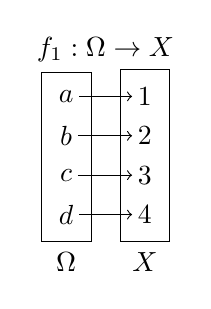
\begin{tikzpicture}[every fit/.style={rectangle,draw,inner sep=1mm,}]
        \node[] (a) at (0,1.5) {$a$};
        \node[] (b) at (0,1.0) {$b$};
        \node[] (c) at (0,0.5) {$c$};
        \node[] (d) at (0,0.0) {$d$};
        \node[] (omega) at (0,-0.6) {$\Omega$};

        \node[] (1) at (1,1.5) {$1$};
        \node[] (2) at (1,1.0) {$2$};
        \node[] (3) at (1,0.5) {$3$};
        \node[] (4) at (1,0.0) {$4$};
        \node[] (x) at (1,-0.6) {$X$};

        \node [] (f) at (0.5,2.1) {$f_1:\Omega \to X$};
        

        \node[draw,fit= (a) (d)] {};
        \node[draw,fit= (1) (4)] {};

        \draw[->,shorten <=-0.5mm,,shorten >=-0.5mm] (a) -- (1) {};
        \draw[->,shorten <=-0.5mm,,shorten >=-0.5mm] (b) -- (2) {};
        \draw[->,shorten <=-0.5mm,,shorten >=-0.5mm] (c) -- (3) {};
        \draw[->,shorten <=-0.5mm,,shorten >=-0.5mm] (d) -- (4) {};

    \end{tikzpicture}
\end{document}